\documentclass[10pt, a4paper]{exam}
\usepackage{graphicx}
\usepackage[a4paper, total={7in, 9.5in}]{geometry}
\usepackage[normalem]{ulem}
\usepackage{amsmath}
\renewcommand\ULthickness{1.0pt}   
\setlength\ULdepth{1.3ex}

\begin{document}


	\noindent
	\begin{minipage}[l]{0.1\textwidth}
		\noindent
		
\includegraphics[width=2.8\textwidth]{ESCUDO.png}
	\end{minipage}
\hfill
\begin{minipage}[c]{0.8\textwidth}
	\begin{center}
		{\large  Departamento de Ingeniería civil y Agrícola\par
		\large	Facultad de Ingeniería	\par
	% \large \textbf{Taller propiedades de los fluidos}	\par
    \large \textbf{Laboratorio No. 1 \\ Conservaci\'on de la energ\'ia}	\par
} %%%%% NOMBRE DEL PROFESOR 
	\end{center}
\end{minipage}
\par
\vspace{0.2in}
\noindent
    \uline{Mecánica de fluidos [2015966]	\hfill 2022-II	}
\par 
\vspace{0.15in}
\noindent

%%%%%%%%%%%%%%%%%%%%%%%%%%%%%
\section{Normas del Laboratorio}
\begin{itemize}
    \item \textbf{Grupos}: Los grupos seran de 5 o 6 estudiantes m\'aximo. Los estudiantes son libres de organizar los grupos.
    \item \textbf{Duraci\'on}: Cada grupo tendr\'a una hora aproxim\'adamente  para realizar el laboratorio.
    \item \textbf{Material}: Es necesario vestir bata o overol para la realizaci\'on del laboratorio. Este atuendo puede ser de cualquier color o fabricante. Traer calculadora, l\'apiz y papel.
\end{itemize}


\section{Objetivo}
En terminos generales, este laboratorio tiene como fin estudiar la conservaci\'on de la energ\'ia en sistemas de flujo a presi\'on en tuber\'ias. Algunos objetivos espec\'ificos propuestos son:
\begin{itemize}
\item Calcular el perfil de la velocidad en una tuber\'ia usando el tubo Pitot y la ecuaci\'on de Bernoulli. Usando el perfil de velocidades, calcular el caudal. 
\item Con base en el perfil de velocidades estimado y la velocidad media en la tuber\'ia, calcular el coeficiente de correci\'on de la energ\'ia cin\'etica o coeficiente de Coriolis.
\item Usando el tubo Venturi y la ecuaci\'on de Bernoulli, calcular el caudal en la tuber\'ia. 
\item Usando la linea de gradiente hidr\'aulico (LGH) y la l\'inea de energ\'ia (LE), estimar las perdidas (por fricci\'on y por accesorios) a lo largo de una tuber\'ia. 
\end{itemize}

\section{Metodolog\'ia}
Este laboratorio se har\'a en dos diferentes experimentos:
\subsection{Experimento 1: Caudal, coeficiente de coriolis y perdidas pro fricci\'on}
Este experimento esta compuesto por un sistema de circulaci\'on de aire a trav\'ez de tres tuber\'ias en paralelo de diferente di\'ametro. Las tuber\'ias poseen man\'ometros conectados a lo largo. La tuber\'ia superior cuenta con un sistema de  tubo Pitot al final para determinar el caudal. La tuber\'ia de retorno en la parte inferior cuenta con un tubo Venturi (ver figura~\ref{exp1}). 
\begin{figure}[h]
    \centering
    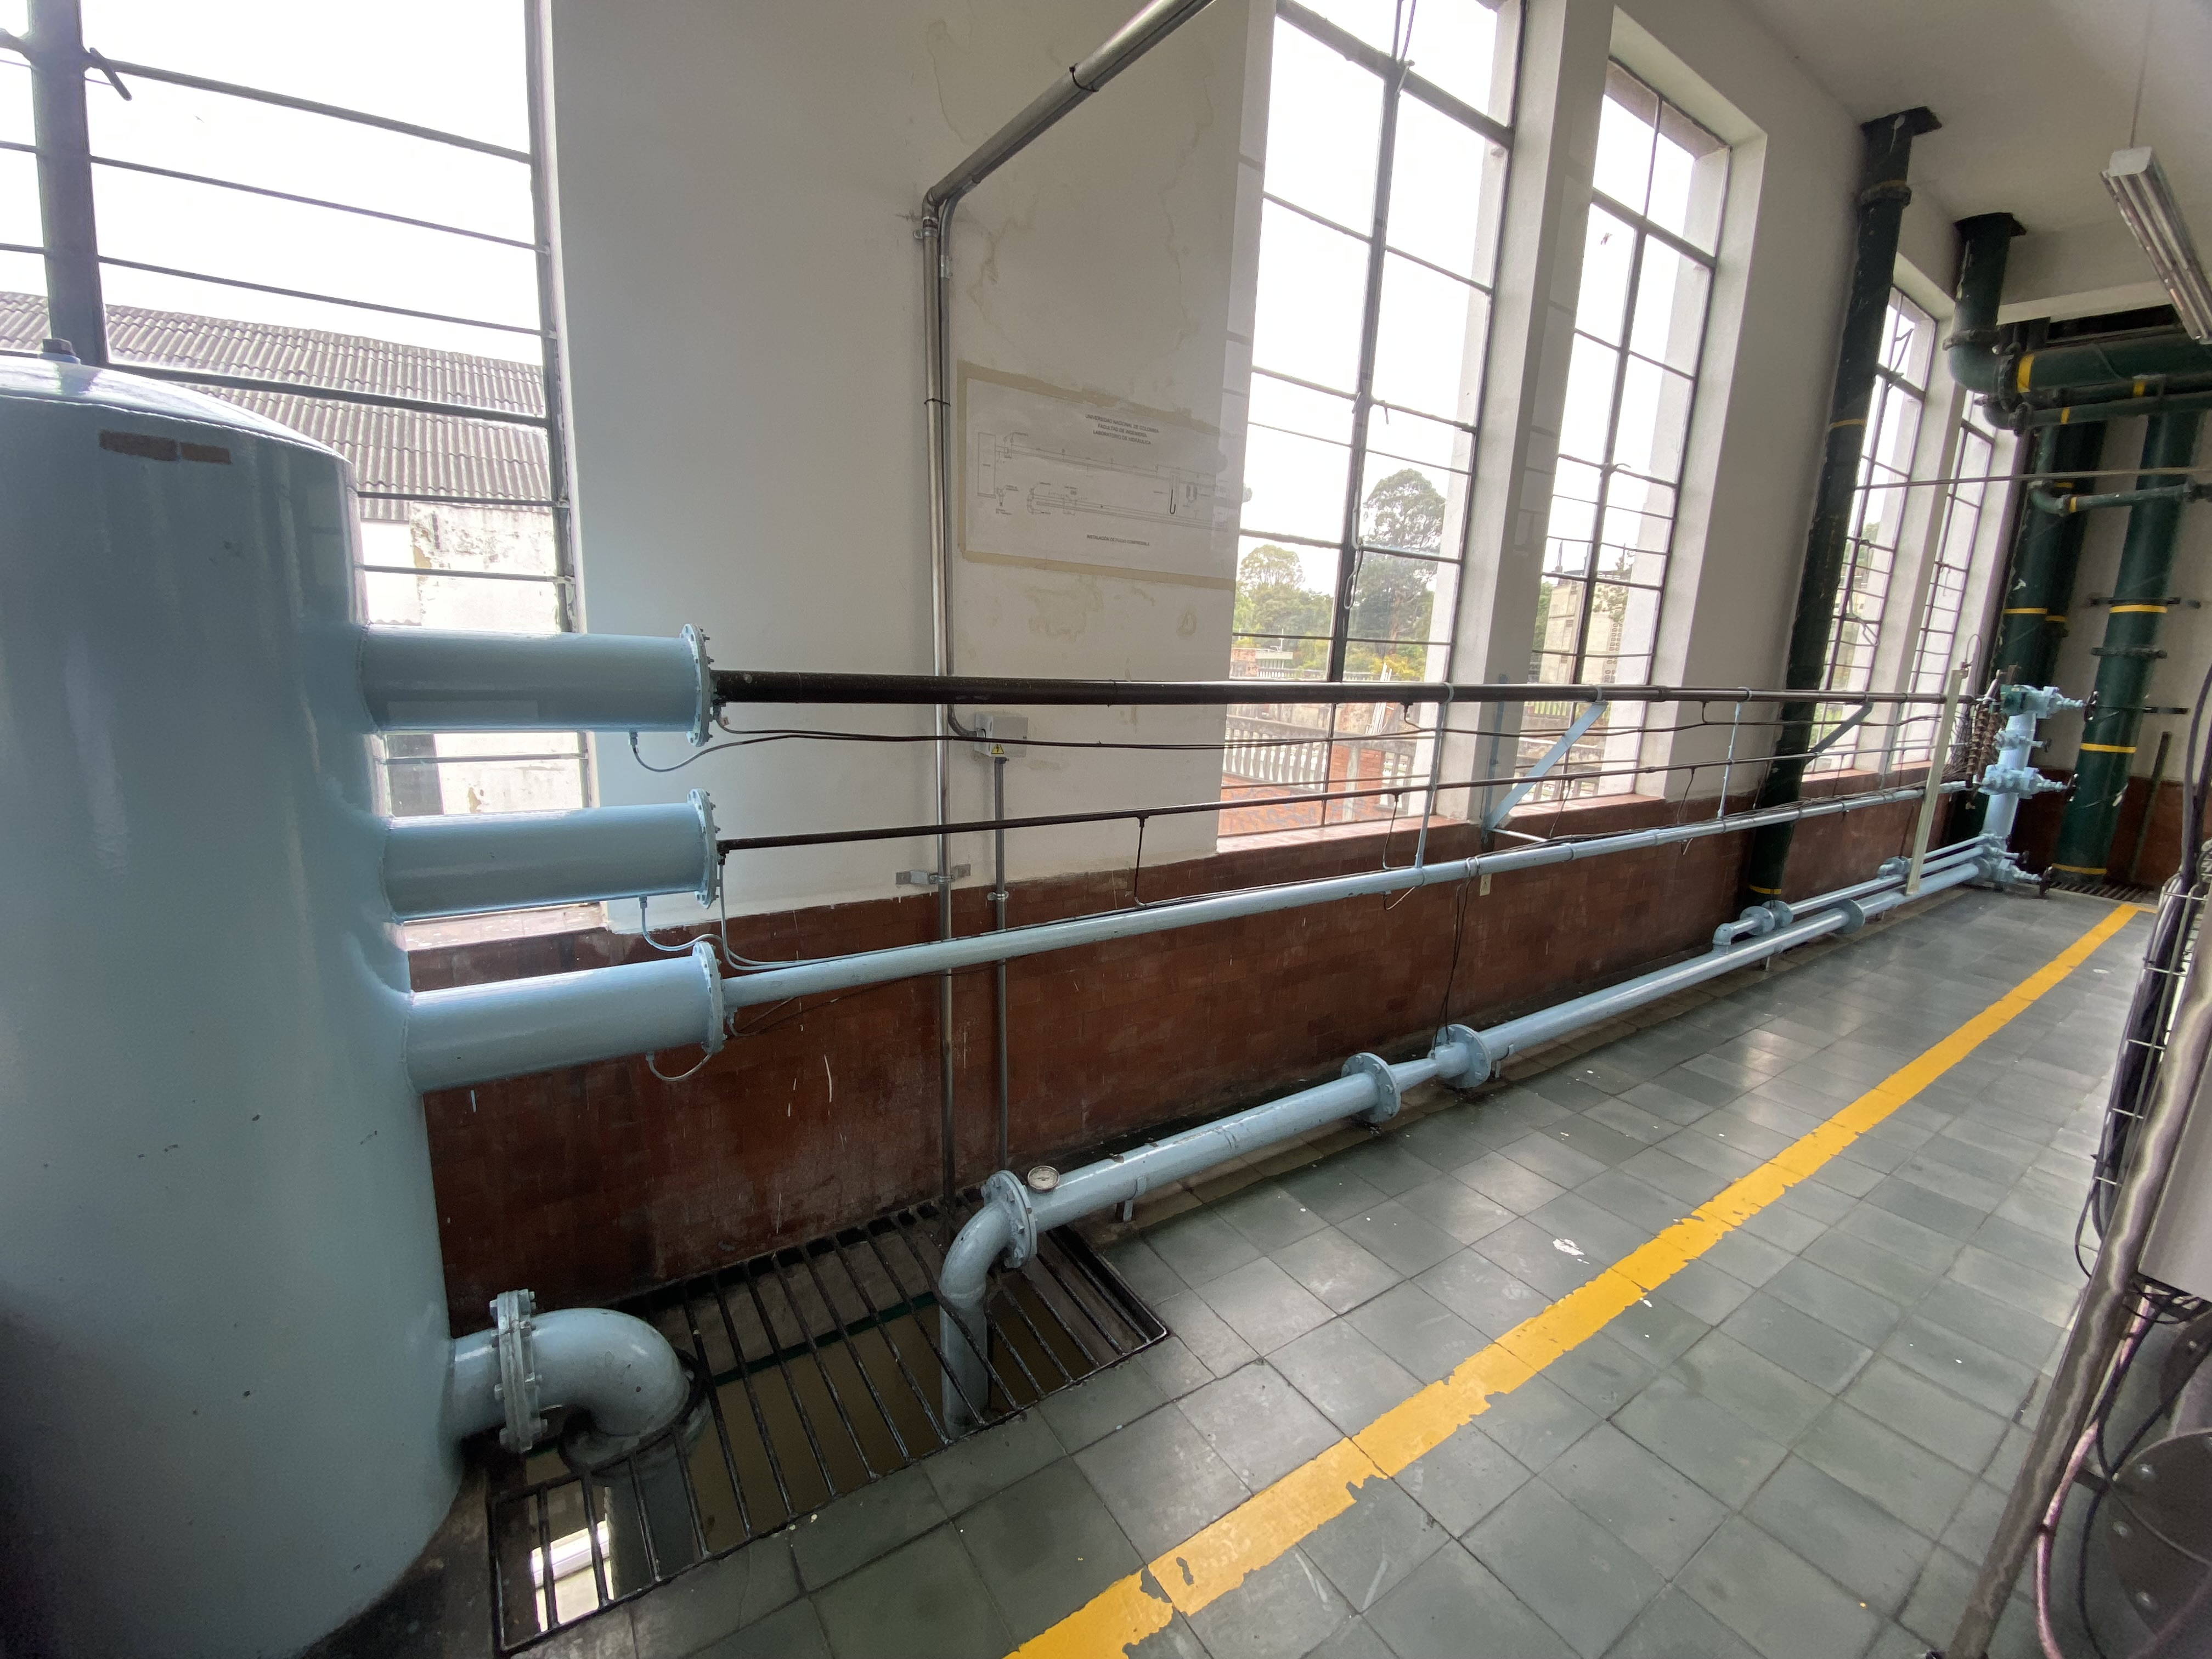
\includegraphics[width=\textwidth]{exp1.jpg}
    \caption{Experimento 1. Flujo de aire en tres tuber\'ias.}
    \label{exp1}
\end{figure}

\subsection{Experimento 2: Perdidas de energ\'ia debido a la fricci\'on y a los accesorios}  
Este experimento esta compuesto por un sistema de dos tuber\'ias en paralelo que transportan agua a presi\'on. Cada tuber\'ia es de diferente material y tienen transiciones bruscas y suaves para cambio de di\'ametro. Cada tuber\'ia tiene una serie de man\'ometros conectados para determinar los cambios de presi\'on debido a la rugosidad o a los accesorios. Un vertedero de cresta delgada es usado para estimar el caudal que circula por cada tuber\'ia (ver figura~\ref{exp2}). 

\begin{figure}[h]
    \centering
    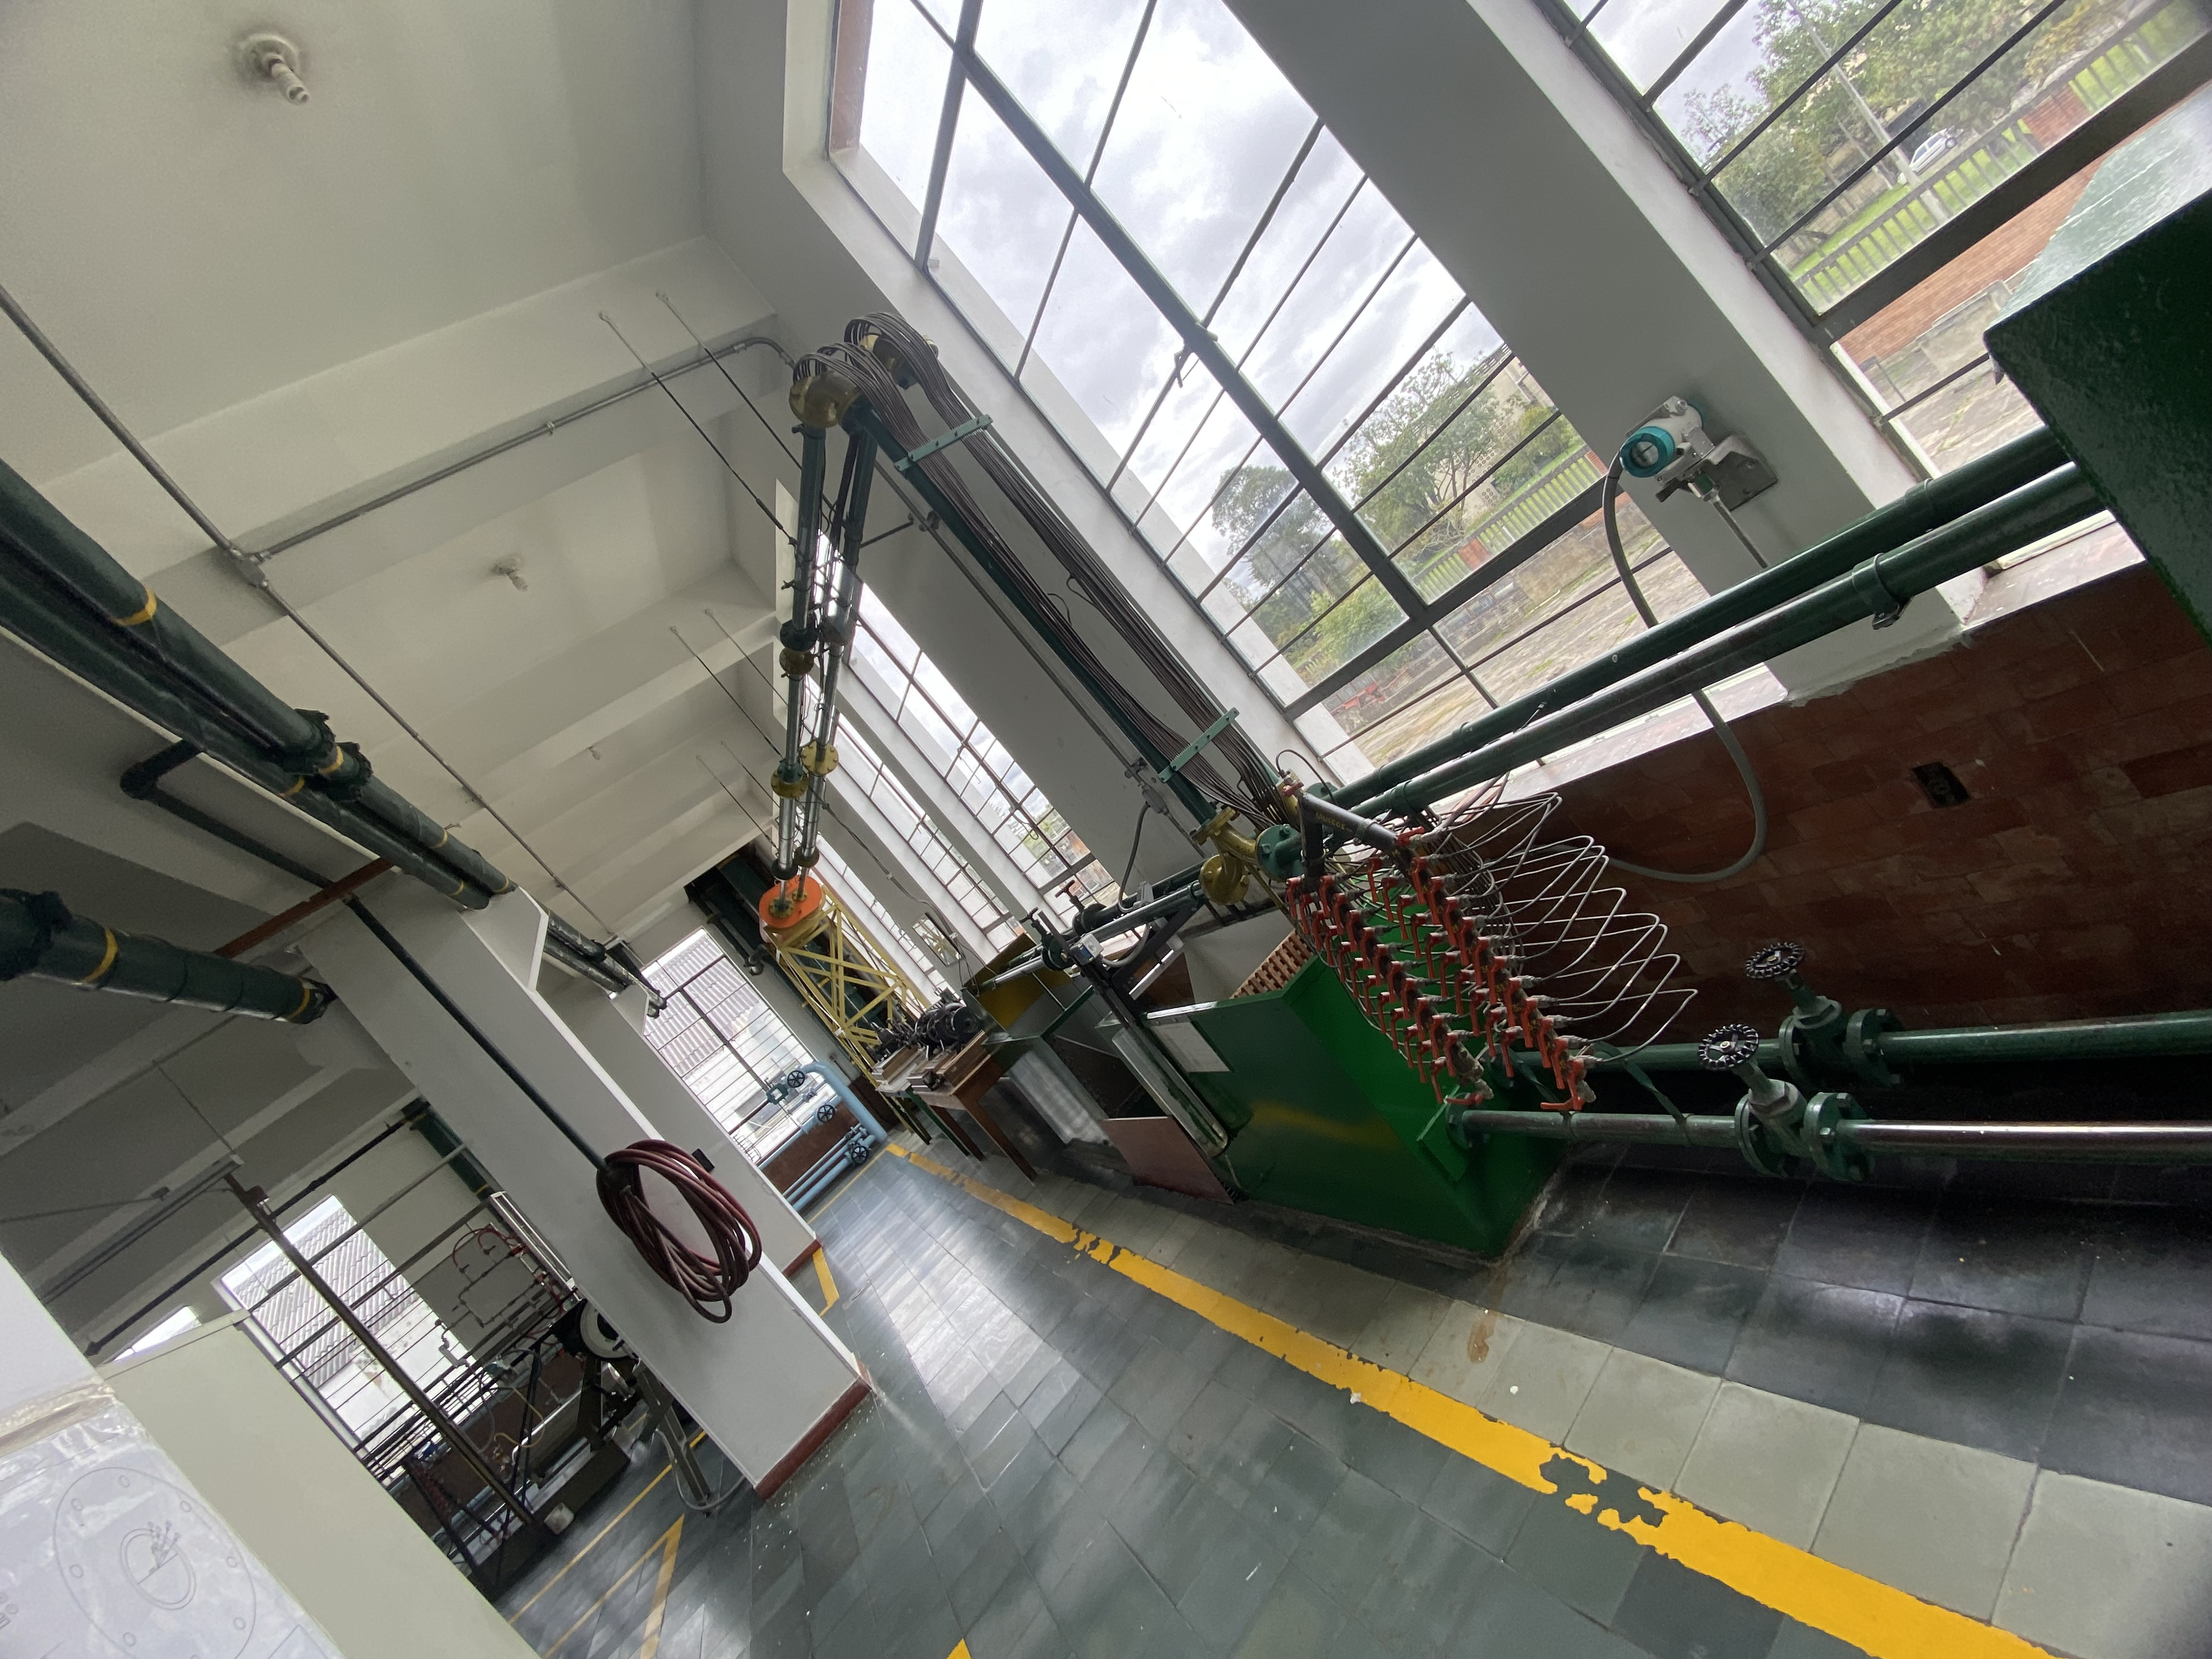
\includegraphics[width=\textwidth]{exp2.jpg}
    \caption{Experimento 2. Flujo de agua en tuber\'ias paralelas con cambios de secci\'on.}
    \label{exp2}
\end{figure}


\section{Resultados esperados}
\subsection{Experimento 1: Caudal, coeficiente de coriolis y perdidas pro fricci\'on}
Para un caudal que aire que circula en la tuber\'ia superior (ver figura~\ref{exp1}), realizar lo siguiente: 
\begin{enumerate}
    \item Usando el tubo Pitot, determinar las velocidades en diferentes puntos de la secci\'on de la tuber\'ia para formar el perfil de velocidades $u$. La velocidad en un punto $i$ de la secci\'on es calculada como:
    $$
    u_1^i = \sqrt{2g \left( \frac{p_2}{\gamma}-\frac{p_1}{\gamma}\right)}
    $$
    donde $p_1$ es la presi\'on medida con el man\'ometro justo antes del tubo Pitot y $p_2$ es la presi\'on medida con el tubo Pitot. Note que $u_2^i \approx 0$ por estanqueidad en la ecuaci\'on de Bernoulli. Este procedimiento se repite para $n$ puntos en la secci\'on transversal de la tuber\'ia.
    \item Una vez se tenga el perfil de velocidades $u$, determinar el caudal como:
    $$
    Q = \sum_{i=1}^n A_i\ u_1^i
    $$
    donde $A_i=2 2\pi r dr$, donde $r$ es la distancia desde el centro al punto de ubicaci\'on del Pitot y $dr$ es el espesor del anillo de area.
    \item Con el perfil de velocidades $u$ y el caudal $Q$, calcular el coeficiente de correcci\'on de la energ\'ia cin\'etica conocido como coeficiente de Coriolis $\alpha$:
    $$
    \alpha = \frac{1}{A} \int_A \left( \frac{u}{V}\right)^3 dA
    $$
    donde $A$ es el \'area transversal de la tuber\'ia y $V$ es la velocidad media del flujo.
    \item Para el caudal calculado, medir las presiones manom\'etricas a lo largo de la tuber\'ia y graficar la LE y la LGH. Determinar las perdidas a lo largo de la tuber\'ia.
    \item Usando el tubo Venturi en la tuberia de retorno inferior (ver figura~\ref{exp1}), calcular el coeficiente de perdidas $C_v$ entre la secci\'on de entrada $1$ y la contracci\'on $2$ usando la ecuaci\'on:
    $$
    Q=V_2 A_2 = C_v A_2 \sqrt{\frac{2g\left(\frac{p_1}{\gamma}-\frac{p_2}{\gamma}\right)}{1-\left(\frac{A_2}{A_1}\right)^2}}
    $$
    Note que el caudal $Q$ es el mismo calculado con el tubo Pitot.
\end{enumerate}
\subsection{Experimento 2: Perdidas de energ\'ia debido a la fricci\'on y a los accesorios}
Para cada una de las tuberias (una con cambios de secci\'on bruscos y otra con cambios suaves), ubicadas en la parte superior (ver figura~\ref{exp2}), determinar para un caudal $Q$ lo siguiente:
\begin{enumerate}
    \item Usando el vertedero de cresta delgada, determinar el caudal que circula por la tuber\'ia. Para esto, se debe medir la distancia desde la cresta del vertedero hasta la superficie libre de agua y luego introducir esta profundidad $h$ en la ecuaci\'on de calibraci\'on del vertedero. 
    \item Usando el n\'umero de Reynolds $NR = \frac{V4R_h}{\nu}$, determinar el tipo de flujo.
    \item Tomar las presiones en cada punto a lo largo de la tuber\'ia. Graficar la LE y la LGH usando todos los puntos de toma de presi\'on.
    \item Calcular las perdidas $h_f$ a lo largo de la tuber\'ia usando la ecuaci\'on de Bernoulli:
    $$
    \frac{p_1}{\gamma}+\frac{\alpha V_1^2}{2g} + z_1 = \frac{p_1}{\gamma}+\frac{\alpha V_1^2}{2g} + z_1 + h_f
    $$
    Asumir $\alpha \approx 1$.
    \item De ser posible, calcular las perdidas en cada uno de los accesorios. A partir de las perdidas totales, determinar cuanta perdida es debido a los accesorios y cuanto a la fricci\'on en la tuber\'ia.
    \item Comparar los resultados de las dos tuber\'ias y discutirlos.
\end{enumerate}


\section{Listado de instrumentos usados}
\begin{enumerate}
\item Medici\'on de presi\'on:
\begin{enumerate}
\item Man\'ometro de agua o de mercurio. El segundo sirve para medir presiones mayores.
\item Man\'ometro Burdon (Mediciones en PSI o columna de Hg)
\item Transductor de presi\'on que reporta los valores en un panel de control.
\end{enumerate}
\item Medici\'on de caudal:
\begin{enumerate}
\item Tubo Pitot: Es un peque\~no tubo en L que se ubica en sentido opuesto al flujo. Es utilizado para medir la velocidad con base en una diferencia de presiones utilizando la ecuaci\'on de Bernoulli. La sumatorio de los valores de las velocidades por el \'area respectiva es igual al caudal de flujo. 
\item Vertedero de cresta delgada: Vertedero triangular que sirve para medir la altura sobre la cresta del vertedero para luego, mediante una ecuaci\'on de calibraci\'on, calcular el caudal.
\item Tubo Venturi: Es un tubo con una reducci\'on r\'apida de la secci\'on transversal que es seguido de una ampliaci\'on gradual de la secci\'on. En la reducci\'on de la linea de gradiente hidr\'aulica cae sustancialmente debido a una disminuci\'on notable de la presi\'on. Utilizando medidas de la presi\'on antes y en la reducci\'on, la ecuaci\'on de Bernoulli y el principio de conservaci\'on de masa es posible calcular el caudal.
\item Medidores de caudal: Instrumentos digit\'ales para medir el caudal.
\end{enumerate}
\end{enumerate}

\section{Informe}
El informe de laboratorio debe contener las siguientes secciones: 
\begin{enumerate}
    \item Introducci\'on: Breve texto para poner en contexto el laboratorio.
    \item Metodolog\'ia: Describe el procedimiento de toma de datos y el seguido para obtener los resultados.
    \item Resultados: Presenta los resultados del labotorio. Dado el caso, se deben incluir gr\'aficas y tablas que resuman los resultados.
    \item Conclusiones: Se discuten all\'i las conclusiones obtenidas a partir de los resultados. Se hacen las comparaciones del caso.
    \item Referencias: Incluir las referencias consultadas.
\end{enumerate}
El informe no debe contener m\'as `de 4 hojas escritas en ambas caras en espacio sencillo, tama\~no de fuente 11 y a doble columna. 

\end{document}



